\begin{enumerate}[label=\thesection.\arabic*,ref=\thesection.\theenumi]
\item  Show that the three lines with direction cosines
$\frac{12}{13},\frac{-3}{13},\frac{-4}{13}$; $\frac{4}{13},\frac{12}{13},\frac{3}{13}$; $\frac{3}{13},\frac{-4}{13},\frac{12}{13}$; are mutually perpendicular.\\
\item  Show that the line through the points $(1,-1,2),(3,4,-2 )$ is perpendicular to the line through the points$(0,3,2)$ and$(3,5,6)$.\\
\item Show that the line through the points $(4,7,8),(2,3,4)$ is parallel to the line through the points $(-1,-2,1),(1,2,5)$.\\
\item  Find the equation of the line which passes through the point $(1,2,3)$ and is parallel to the vector $3\hat{i}+2\hat{j}-2\hat{k}$\\
\item  Find the equation of the line in vector and in cartesian form that passes through the point with position vector $2\hat{i}-\hat{j}+4\hat{k}$ and is in direction $\hat{i}+2\hat{j}-\hat{k}$.\\
\item Find the cartesian equation of the line which passes through the point $(-2,4,-5)$ and parallel to the line given by$ \frac{x+3}{3}=\frac{y-4}{5}=\frac{z+8}{6}$.\\
\item The cartesian equation of a line is $ \frac{x-5}{3}=\frac{y+4}{7}=\frac{z-6}{2}$. Write its vector form.\\
\item Find the vector and the cartesian equations of the lines that passes through the origin and $(5,-2,3)$.\\
\item Find the vector and the cartesian equations of the line that passes through the points $(3,-2,-5),(3,-2,6)$.\\
\item  Find the angle between the following pairs of lines:
\begin{enumerate}
\item  $\overrightarrow{r}=2\hat{i}-5\hat{j}+\hat{k}+\lambda(3\hat{i}+2\hat{j}+6\hat{k})$ and\\ $\overrightarrow{r}=7\hat{i}-6\hat{k}+\mu(\hat{i}+2\hat{j}+2\hat{k})$
\item   $\overrightarrow{r}=3\hat{i}+\hat{j}-2\hat{k}+\lambda(\hat{i}-\hat{j}-2\hat{k})$ and\\ $\overrightarrow{r}=2\hat{i}-\hat{j}-56\hat{k}+\mu(3\hat{i}-5\hat{j}-4\hat{k})$ 
\end{enumerate}
\item Find the angle between the following pairs of lines:
\begin{enumerate}
\item $ \frac{x-2}{2}=\frac{y-1}{5}=\frac{z+3}{-3}$ and $ \frac{x+2}{-1}=\frac{y-4}{8}=\frac{z-5}{4}$.
\item $ \frac{x}{2}=\frac{y}{2}=\frac{z}{1}$ and $ \frac{x-5}{4}=\frac{y-2}{1}=\frac{z-3}{8}$.
\end{enumerate}
\item Find the values of p so that the lines $ \frac{1-x}{3}=\frac{7y-14}{2p}=\frac{z-3}{2}$ and $ \frac{7-7x}{3p}=\frac{y-5}{1}=\frac{6-z}{5}$ are at right angles.
\item Show that the lines $ \frac{x-5}{7}=\frac{y+2}{-5}=\frac{z}{1}$ and $ \frac{x}{1}=\frac{y}{2}=\frac{z}{3}$ are perpendicular to each other.
\item Find the shortest distance between the lines\\  $\overrightarrow{r}=(\hat{i}+2\hat{j}+\hat{k})+\lambda(\hat{i}-\hat{j}+\hat{k})$ and \\$\overrightarrow{r}=2\hat{i}-\hat{j}-\hat{k}+\mu(2\hat{i}+\hat{j}+2\hat{k})$
\item Find the shortest distance between the lines\\
$ \frac{x+1}{7}=\frac{y+1}{-6}=\frac{z+1}{1}$ and $ \frac{x-3}{1}=\frac{y-5}{-2}=\frac{z-7}{1}$ 
    \item Find the shortest distance between the lines whose vector equations are
    \begin{align}
        \vec{x} = \myvec{1\\2\\3} + \lambda_1\myvec{1\\-3\\2}
        \label{eq:chapters/12/11/2/16/L1}
    \end{align}
    and
    \begin{align}
        \vec{x} = \myvec{4\\5\\6} + \lambda_2\myvec{2\\3\\1}
        \label{eq:chapters/12/11/2/16/L2}
    \end{align}
    \solution
		\iffalse
\documentclass[journal,12pt,twocolumn]{IEEEtran}
\usepackage{setspace}
\usepackage{gensymb}
\usepackage{xcolor}
\usepackage{caption}
\singlespacing
\usepackage{siunitx}
\usepackage[cmex10]{amsmath}
\usepackage{mathtools}
\usepackage{hyperref}
\usepackage{amsthm}
\usepackage{mathrsfs}
\usepackage{txfonts}
\usepackage{stfloats}
\usepackage{cite}
\usepackage{cases}
\usepackage{subfig}
\usepackage{longtable}
\usepackage{multirow}
\usepackage{enumitem}
\usepackage{bm}
\usepackage{mathtools}
\usepackage{listings}
\usepackage{tikz}
\usetikzlibrary{shapes,arrows,positioning}
\usepackage{circuitikz}
\renewcommand{\vec}[1]{\boldsymbol{\mathbf{#1}}}
\DeclareMathOperator*{\Res}{Res}
\renewcommand\thesection{\arabic{section}}
\renewcommand\thesubsection{\thesection.\arabic{subsection}}
\renewcommand\thesubsubsection{\thesubsection.\arabic{subsubsection}}

\renewcommand\thesectiondis{\arabic{section}}
\renewcommand\thesubsectiondis{\thesectiondis.\arabic{subsection}}
\renewcommand\thesubsubsectiondis{\thesubsectiondis.\arabic{subsubsection}}
\hyphenation{op-tical net-works semi-conduc-tor}

\lstset{
language=Python,
frame=single, 
breaklines=true,
columns=fullflexible
}
\begin{document}
\theoremstyle{definition}
\newtheorem{theorem}{Theorem}[section]
\newtheorem{problem}{Problem}
\newtheorem{proposition}{Proposition}[section]
\newtheorem{lemma}{Lemma}[section]
\newtheorem{corollary}[theorem]{Corollary}
\newtheorem{example}{Example}[section]
\newtheorem{definition}{Definition}[section]
\newcommand{\BEQA}{\begin{eqnarray}}
\newcommand{\EEQA}{\end{eqnarray}}
\newcommand{\define}{\stackrel{\triangle}{=}}
\newcommand{\myvec}[1]{\ensuremath{\begin{pmatrix}#1\end{pmatrix}}}
\newcommand{\mydet}[1]{\ensuremath{\begin{vmatrix}#1\end{vmatrix}}}
\bibliographystyle{IEEEtran}
\providecommand{\nCr}[2]{\,^{#1}C_{#2}} % nCr
\providecommand{\nPr}[2]{\,^{#1}P_{#2}} % nPr
\providecommand{\mbf}{\mathbf}
\providecommand{\pr}[1]{\ensuremath{\Pr\left(#1\right)}}
\providecommand{\qfunc}[1]{\ensuremath{Q\left(#1\right)}}
\providecommand{\sbrak}[1]{\ensuremath{{}\left[#1\right]}}
\providecommand{\lsbrak}[1]{\ensuremath{{}\left[#1\right.}}
\providecommand{\rsbrak}[1]{\ensuremath{{}\left.#1\right]}}
\providecommand{\brak}[1]{\ensuremath{\left(#1\right)}}
\providecommand{\lbrak}[1]{\ensuremath{\left(#1\right.}}
\providecommand{\rbrak}[1]{\ensuremath{\left.#1\right)}}
\providecommand{\cbrak}[1]{\ensuremath{\left\{#1\right\}}}
\providecommand{\lcbrak}[1]{\ensuremath{\left\{#1\right.}}
\providecommand{\rcbrak}[1]{\ensuremath{\left.#1\right\}}}
\theoremstyle{remark}
\newtheorem{rem}{Remark}
\newcommand{\sgn}{\mathop{\mathrm{sgn}}}
\newcommand{\rect}{\mathop{\mathrm{rect}}}
\newcommand{\sinc}{\mathop{\mathrm{sinc}}}
\providecommand{\abs}[1]{\left\vert#1\right\vert}
\providecommand{\res}[1]{\Res\displaylimits_{#1}} 
\providecommand{\norm}[1]{\lVert#1\rVert}
\providecommand{\mtx}[1]{\mathbf{#1}}
\providecommand{\mean}[1]{E\left[ #1 \right]}
\providecommand{\fourier}{\overset{\mathcal{F}}{ \rightleftharpoons}}
\providecommand{\ztrans}{\overset{\mathcal{Z}}{ \rightleftharpoons}}
\providecommand{\system}[1]{\overset{\mathcal{#1}}{ \longleftrightarrow}}
\newcommand{\solution}{\noindent \textbf{Solution: }}
\providecommand{\dec}[2]{\ensuremath{\overset{#1}{\underset{#2}{\gtrless}}}}
\let\StandardTheFigure\thefigure
\def\putbox#1#2#3{\makebox[0in][l]{\makebox[#1][l]{}\raisebox{\baselineskip}[0in][0in]{\raisebox{#2}[0in][0in]{#3}}}}
     \def\rightbox#1{\makebox[0in][r]{#1}}
     \def\centbox#1{\makebox[0in]{#1}}
     \def\topbox#1{\raisebox{-\baselineskip}[0in][0in]{#1}}
     \def\midbox#1{\raisebox{-0.5\baselineskip}[0in][0in]{#1}}

\vspace{3cm}
\title{Line Assignment}
\author{Gautam Singh}
\maketitle
\bigskip

\begin{abstract}
    This document contains the solution to Question 16 of Exercise 2 in Chapter
    11 of the class 12 NCERT textbook.
\end{abstract}
\fi
    In this case,
    \begin{align}
        \vec{x_1} = \myvec{1\\2\\3} \quad \vec{x_2} = \myvec{4\\5\\6}
        \quad \vec{m_1} = \myvec{1\\-3\\2} \quad \vec{m_2} = \myvec{2\\3\\1}
        \label{eq:chapters/12/11/2/16/vals}
    \end{align}
    To check whether \eqref{eq:chapters/12/11/2/16/intersect-cond} has a solution in $\vec{\lambda}$,
    we use the augmented matrix.
    \begin{align}
        \myvec{1&2&3\\-3&3&3\\2&1&3} &\xleftrightarrow[]{R_2\leftarrow R_2+3R_1} \myvec{1&2&3\\0&9&12\\2&1&3} \\
                &\xleftrightarrow[]{R_3\leftarrow R_3-2R_1} \myvec{1&2&3\\0&9&12\\0&-3&-3} \\
                &\xleftrightarrow[]{R_3\leftarrow 3R_3+R_2} \myvec{1&2&3\\0&9&12\\0&0&3}
                \label{eq:chapters/12/11/2/16/rank-aug}
    \end{align}
    Clearly, the rank of this matrix is 3, and therefore, the lines are skew.
%
    Substituting from \eqref{eq:chapters/12/11/2/16/vals} in \eqref{eq:chapters/12/11/2/16/lambda-eqn} and forming the 
    augmented matrix,
    \begin{align}
        \myvec{14&-5&0\\-5&14&18} &\xleftrightarrow[]{R_1\leftarrow R_1+R_2} \myvec{9&9&18\\-5&14&18} \\
                 &\xleftrightarrow[]{R_1\leftarrow\frac{R_1}{9}} \myvec{1&1&2\\-5&14&18} \\
                 &\xleftrightarrow[]{R_2\leftarrow R_2+5R_1} \myvec{1&1&2\\0&19&28} \\
                 &\xleftrightarrow[]{R_1\leftarrow19R_1-R_2} \myvec{19&0&10\\0&19&28} \\
                 &\xleftrightarrow[]{\substack{R_1\leftarrow\frac{R_1}{19}\\R_2\leftarrow\frac{R_2}{9}}}
                    \myvec{1&0&\frac{10}{19}\\0&1&\frac{28}{19}} \\
                    \implies \vec{\lambda} &= \frac{1}{19}\myvec{10\\28}
        \label{eq:chapters/12/11/2/16/lambda-sol}
    \end{align}
    Hence, using \eqref{eq:chapters/12/11/2/16/lambda-def} and substituing into \eqref{eq:chapters/12/11/2/16/a-def} and \eqref{eq:chapters/12/11/2/16/b-def},
    \begin{align}
        \vec{A} = \frac{1}{19}\myvec{29\\8\\77} \quad \vec{B} = \frac{1}{19}\myvec{20\\11\\86}
    \end{align}
    Thus, the required distance is
    \begin{align}
        \norm{\vec{B}-\vec{A}} = \frac{\sqrt{9^2 +3^2 +(-9)^2}}{19} = \frac{3}{\sqrt{19}}
    \end{align}
    The situation is depicted in Fig. \ref{fig:chapters/12/11/2/16/skew}.

    \begin{figure}[!ht]
        \centering
        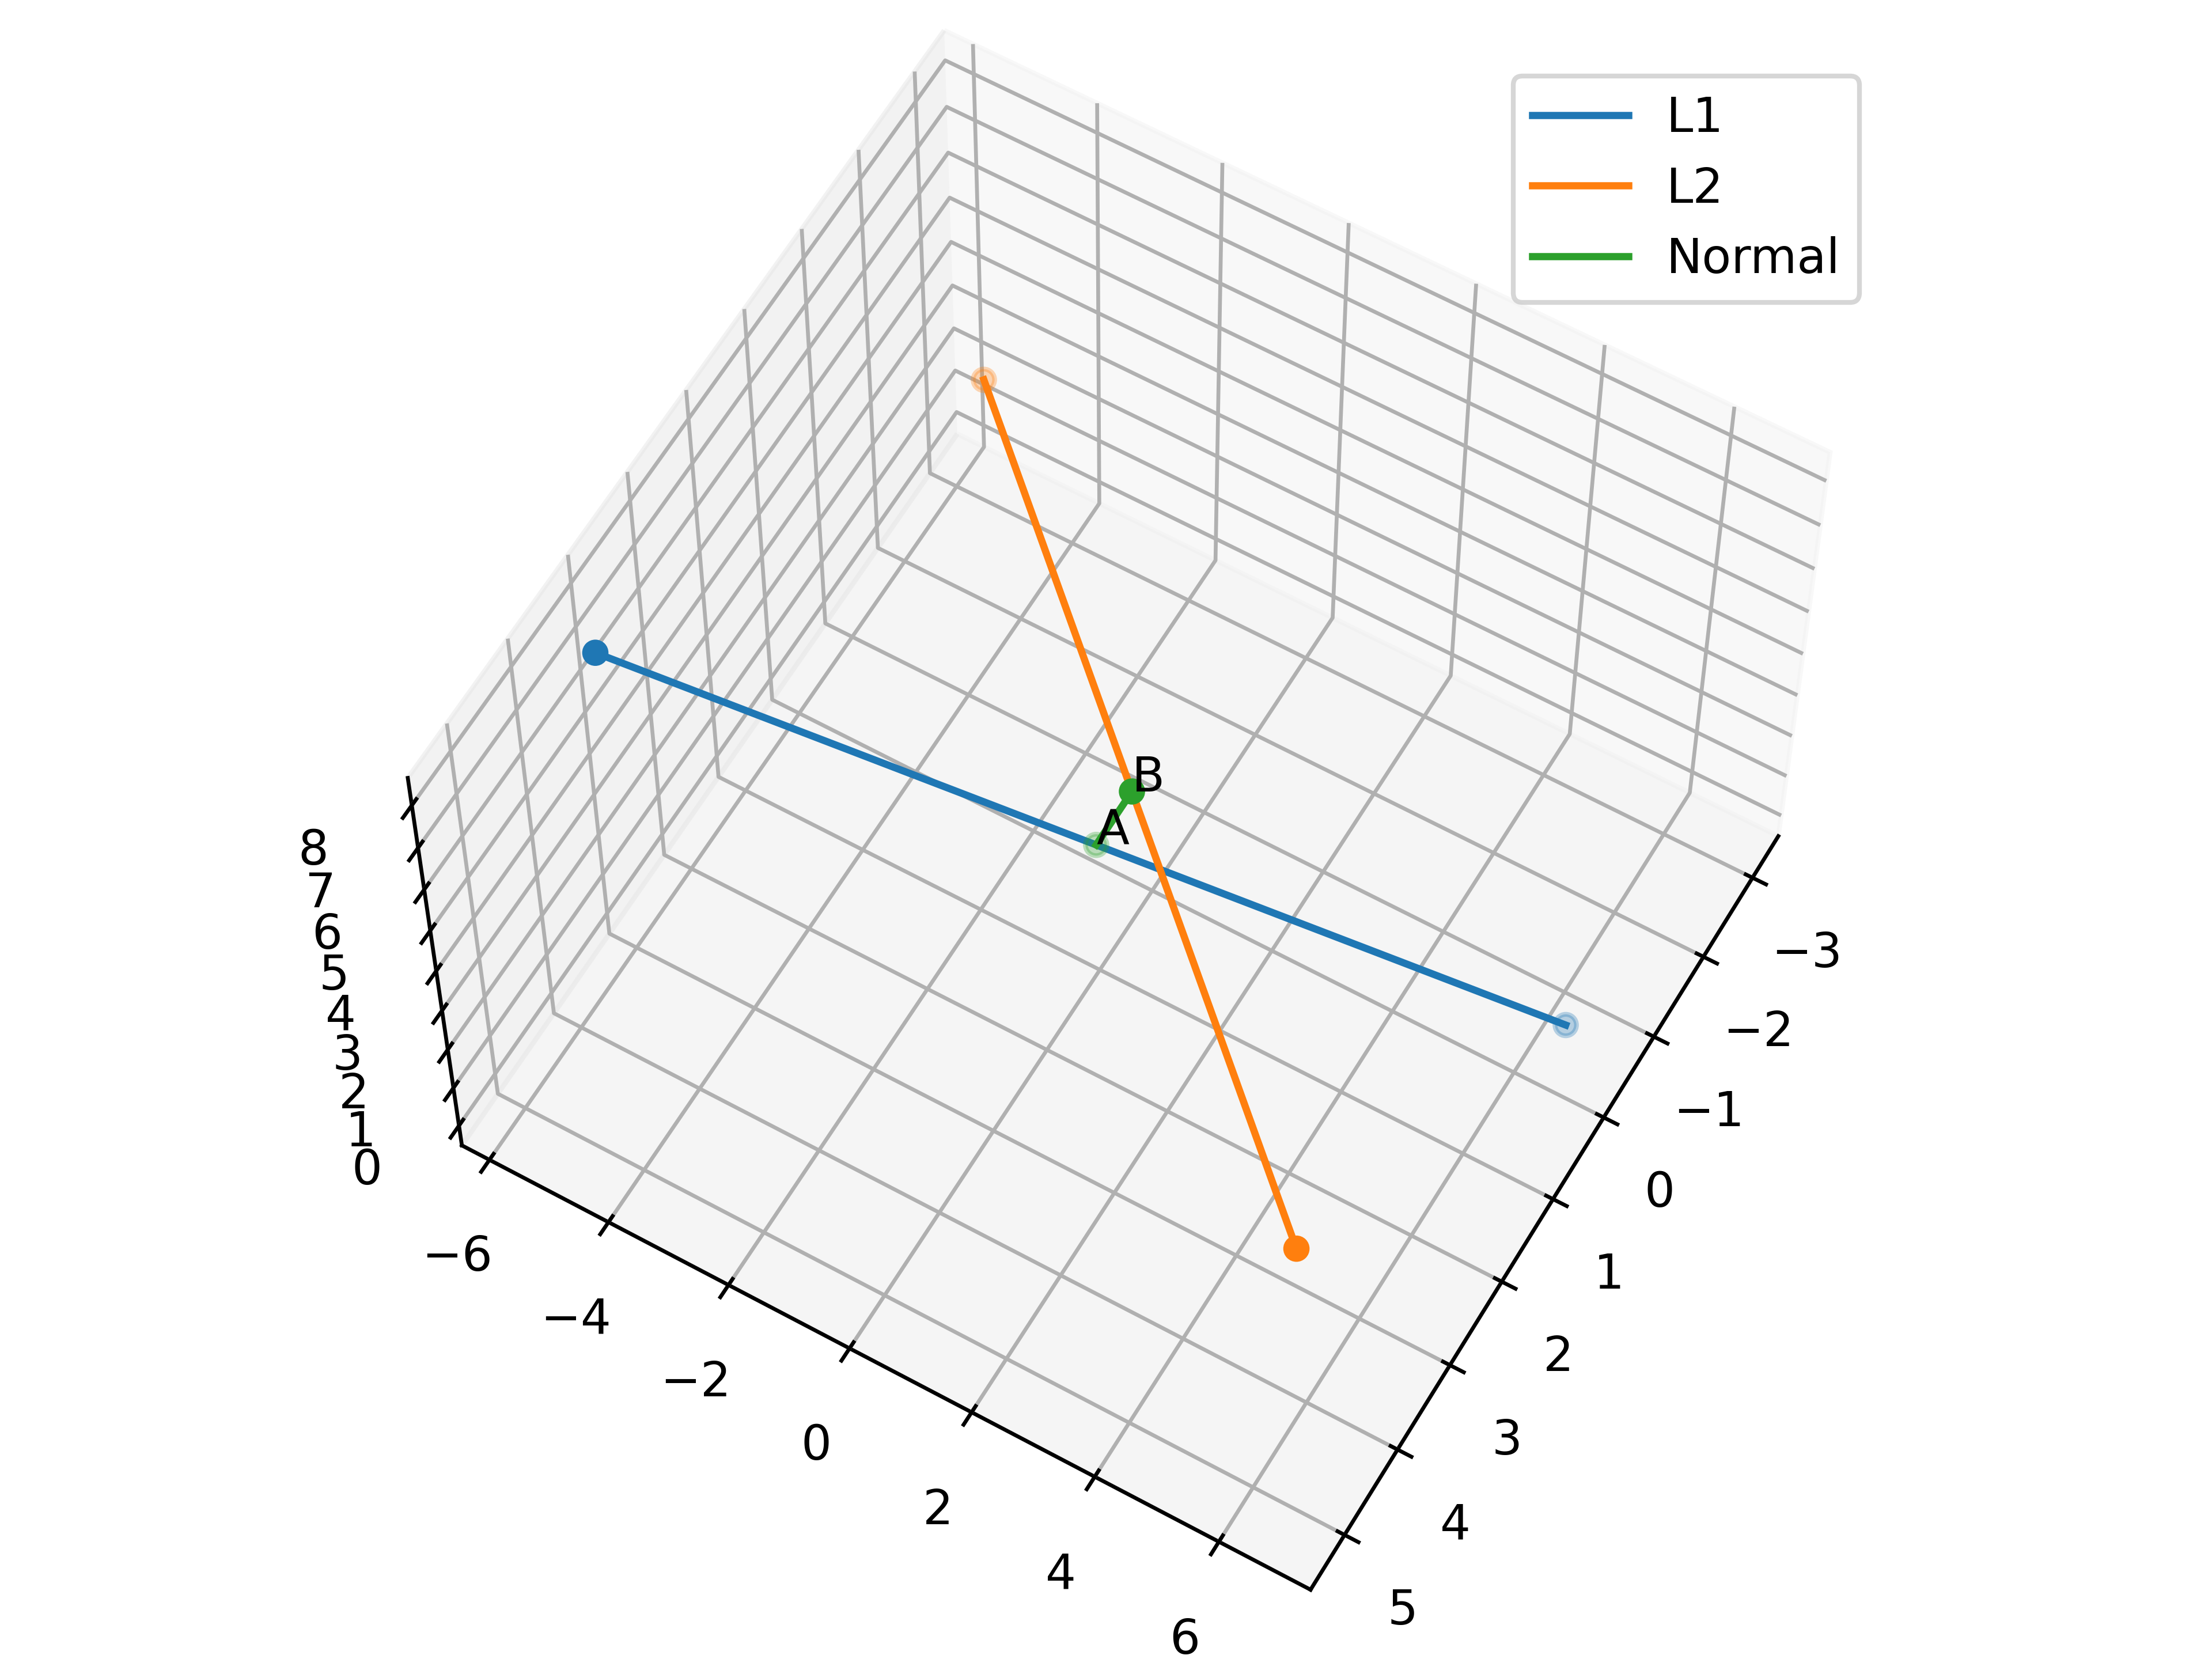
\includegraphics[width=\columnwidth]{chapters/12/11/2/16/figs/skew.png}
        \caption{$AB$ is the required shortest distance.}
        \label{fig:chapters/12/11/2/16/skew}
    \end{figure}

\item Find the shortest distance between the lines whose vector equations are \\
 $\overrightarrow{r}=(1-t)\hat{i}+(t-2)\hat{j}+(3-2t)\hat{k}$     and  \\$\overrightarrow{r}=(s+1)\hat{i}+(2s-1)\hat{j}-(2s+1)\hat{k}$
\end{enumerate}

